% =========================================================================
% MEMORIA DEL PROYECTO - Depreciación del euro (2010-2025)
% =========================================================================

\documentclass{article}

\usepackage{microtype}
\usepackage{graphicx}
\graphicspath{{docs/img/}{../img/}}
\usepackage{caption}
\captionsetup{font=small,labelfont=bf}
\usepackage[utf8]{inputenc}
\usepackage{csquotes}
\usepackage{booktabs}
\usepackage{hyperref}
\hypersetup{colorlinks=true,linkcolor=blue,citecolor=blue,urlcolor=cyan}
\newcommand{\theHalgorithm}{\arabic{algorithm}}
\usepackage[accepted]{icml2025}
\usepackage[T1]{fontenc}
\usepackage[spanish,es-tabla,es-noshorthands]{babel}
\usepackage{listings}
\usepackage{xcolor}
\usepackage{float}
\usepackage{array}

\definecolor{codegreen}{rgb}{0,0.6,0}
\definecolor{codegray}{rgb}{0.5,0.5,0.5}
\definecolor{backcolour}{rgb}{0.95,0.95,0.92}

\lstset{
    backgroundcolor=\color{backcolour},
    basicstyle=\ttfamily\footnotesize,
    breaklines=true,
    captionpos=b,
    keepspaces=true,
    showstringspaces=false,
    tabsize=2
}

\icmltitlerunning{Depreciacion del euro y erosion del poder adquisitivo en Espana (2010-2025)}

\begin{document}

\twocolumn[
\icmltitle{Depreciacion del euro y erosion del poder adquisitivo en Espana (2010-2025)}
\icmlsetsymbol{equal}{*}
\begin{icmlauthorlist}
\icmlauthor{Alejandro Martinez}{ua}
\icmlauthor{Alejandro Parra}{ua}
\icmlauthor{Mauro Carles}{ua}
\icmlauthor{Jordi Blasco}{ua}
\end{icmlauthorlist}
\icmlaffiliation{ua}{Escuela Politecnica Superior, Universidad de Alicante. Asignatura: Adquisicion y Preparacion de Datos. Grado en Ingenieria en Inteligencia Artificial.}
\icmlcorrespondingauthor{Grupo de Practicas}{}
\icmlkeywords{Inflacion, Poder Adquisitivo, Euro, Datos, ETL, Visualizacion}
\vskip 0.3in
]

\printAffiliationsAndNotice{}

\begin{abstract}
Este proyecto analiza la erosion del poder adquisitivo en Espana durante el periodo 2010-2025, integrando datos macroeconomicos, salariales y financieros. Mediante la construccion de un almacen de datos (Data Warehouse) con arquitectura en estrella y procesos ETL robustos, se demuestra la divergencia entre la inflacion oficial (IPC) y la depreciacion real del euro frente a activos refugio como el oro. El estudio ofrece una vision critica sobre la ``inflacion oculta'' y la desigualdad patrimonial.
\end{abstract}

% =========================================================================
% SECCION 1: DEFINICION DEL PROYECTO
% =========================================================================
\section{Definicion del proyecto centrado en los datos}

\subsection{Introduccion y contexto economico}
Durante el periodo 2010-2025, la economía española ha atravesado múltiples crisis que han impactado profundamente en el bienestar de los hogares. El periodo comenzó con las secuelas de la crisis financiera de 2008, continuó con la crisis de deuda europea (2010-2012), experimentó una recuperación moderada (2014-2019), enfrentó el shock de la pandemia COVID-19 (2020-2021), y recientemente ha vivido un repunte inflacionario sin precedentes (2021-2024) motivado por disrupciones en cadenas de suministro y tensiones geopolíticas.

Este proyecto surge de una observación crítica: \textbf{las cifras oficiales de inflación (IPC) no capturan completamente la erosión del poder adquisitivo real de los ciudadanos}. Mientras el IPC oficial ha mostrado tasas moderadas en la mayor parte del periodo (con excepciones puntuales), otros indicadores económicos revelan una historia diferente:

\begin{itemize}
    \item El \textbf{euro ha perdido valor} frente al dólar estadounidense de forma significativa
    \item Los \textbf{salarios nominales}han crecido por debajo de la inflación en muchos años
    \item Los \textbf{activos refugio} como el oro han experimentado revalorizaciones masivas
    \item La \textbf{brecha de desigualdad} se ha ampliado, no solo en ingresos, sino especialmente en patrimonio acumulado
\end{itemize}

Este fenómeno, que algunos economistas denominan \textbf{``inflacion oculta''}, se manifiesta cuando medimos el bienestar económico no en euros nominales, sino en capacidad real de adquisición de bienes, servicios y activos tangibles.

\subsection{Problematica y motivacion}
La problemática central que aborda este proyecto se puede resumir en las siguientes preguntas:

Esta pregunta esconde multiples dimensiones:
\begin{itemize}
    \item \textbf{Dimension monetaria:} Cuanto valor ha perdido el euro?
    \item \textbf{Dimension laboral:} Han crecido los salarios al ritmo de los precios?
    \item \textbf{Dimension patrimonial:} Que estrategias han protegido mejor el patrimonio?
    \item \textbf{Dimension social:} Se ha ampliado la brecha entre quienes tienen acceso a activos refugio?
\end{itemize}

La motivacion es \textbf{cuantificar con datos objetivos} estas dimensiones, integrando datos macroeconomicos (INE, BCE), mercados financieros (bolsa, oro), distribucion salarial por deciles y simulaciones de acumulacion patrimonial.

\subsection{Preguntas de investigacion}
Para estructurar el analisis, definimos cinco preguntas especificas:

\textbf{Pregunta 1: Evolucion de activos vs. efectivo}\\
Como ha evolucionado el valor real de 100EUR en diferentes activos (efectivo, oro, IBEX-35, salario medio) durante 2010-2025, ajustado por inflacion?

\textbf{Pregunta 2: Inflacion oculta medida en oro}\\
Cual es la ``inflacion oculta'' si medimos el salario medio en onzas de oro en lugar de euros nominales?

\textbf{Pregunta 3: Rendimientos reales por activo}\\
Que activos han ofrecido rendimientos reales positivos de forma consistente durante 2010-2025?

\textbf{Pregunta 4: Impacto de la capacidad de ahorro por decil salarial}\\
Como afecta la capacidad de ahorro y la estrategia de inversion a la acumulacion de patrimonio segun el decil salarial?

\textbf{Pregunta 5: Desigualdad salarial vs. patrimonial}\\
En que medida la brecha de desigualdad patrimonial supera a la brecha salarial debido al acceso diferencial a activos refugio?

\subsection{Objetivos del proyecto}

\textbf{Objetivos academicos:}
\begin{enumerate}
    \item Integracion de fuentes heterogeneas (CSV, APIs)
    \item Diseno de almacen de datos analitico (modelo estrella)
    \item Proceso ETL reproducible (Pentaho + Python)
    \item Transformacion semantica (Schema.org JSON-LD)
    \item Visualizacion orientada a insight
\end{enumerate}

\textbf{Objetivos tecnicos:}
\begin{enumerate}
    \item Automatizacion de descarga de datos (\texttt{descarga\_datasets.py})
    \item Limpieza robusta de datos
    \item Base de datos contenedorizada (Docker MySQL)
    \item Modelo dimensional escalable
    \item Exportacion de datos procesados
\end{enumerate}

\textbf{Objetivos analiticos:}
\begin{enumerate}
    \item Cuantificar la inflacion oculta
    \item Identificar activos refugio efectivos
    \item Visualizar la desigualdad patrimonial
    \item Simular escenarios realistas
\end{enumerate}

\subsection{Casos de uso}

\textbf{Caso 1: Analisis de portafolios para particulares}\\
Actor: Ciudadano con capacidad de ahorro. Objetivo: Decidir como distribuir ahorros.

\textbf{Caso 2: Investigacion economica}\\
Actor: Economista o investigador. Objetivo: Analizar evolucion de desigualdad patrimonial.

\textbf{Caso 3: Educacion financiera}\\
Actor: Docente de economia. Objetivo: Explicar inflacion e inversion con datos reales.

\textbf{Caso 4: Auditoria de politicas publicas}\\
Actor: Analista de politicas. Objetivo: Evaluar efectividad de politicas salariales.

% =========================================================================
% SECCION 2: ANALISIS DE NECESIDADES DE DATOS
% =========================================================================
\section{Analizar y evaluar necesidades de datos}

\subsection{Metodologia de seleccion de datos}
La seleccion siguio tres fases:

\textbf{Fase 1: Identificacion de dominios clave}
\begin{enumerate}
    \item Precios y inflacion $\to$ IPC del INE
    \item Mercado laboral $\to$ Salarios y empleo del INE
    \item Mercados financieros $\to$ IBEX-35 (Yahoo Finance)
    \item Activos refugio $\to$ Oro (Yahoo Finance)
    \item Tipos de cambio $\to$ EUR/USD (Yahoo Finance)
\end{enumerate}

\textbf{Fase 2: Evaluacion de fuentes}\\
Criterios: oficialidad, cobertura temporal (2010-2025), granularidad, accesibilidad, formato estructurado.

\textbf{Fase 3: Validacion cruzada}\\
Contraste entre fuentes (ej. EUR/USD de Yahoo vs BCE).

\subsection{Datasets seleccionados}

\textbf{Dataset 1: IPC (Indice de Precios al Consumo)}\\
Fuente: INE. Frecuencia: Anual. Cobertura: 2010-2021.\\
Justificacion: Indicador oficial para deflactar valores nominales.

\textbf{Dataset 2: Salarios}\\
Fuente: INE (Encuesta Estructura Salarial). Frecuencia: Anual/Mensual.\\
Justificacion: Principal fuente de ingresos. Permite analizar desigualdad por deciles.

\textbf{Dataset 3: Empleo y desempleo}\\
Fuente: INE (EPA). Frecuencia: Trimestral.\\
Justificacion: Contexto laboral (temporalidad, desempleo juvenil).

\textbf{Dataset 4: IBEX-35}\\
Fuente: Yahoo Finance (\texttt{\^{}IBEX}). Frecuencia: Diaria.\\
Justificacion: Representa inversion en renta variable espanola.

\textbf{Dataset 5: Oro (precio en USD)}\\
Fuente: Yahoo Finance (\texttt{GC=F}). Frecuencia: Diaria.\\
Justificacion: Activo refugio por excelencia. Se convierte a EUR.

\textbf{Dataset 6: Tipo de cambio EUR/USD}\\
Fuente: Yahoo Finance (\texttt{EURUSD=X}). Frecuencia: Diaria.\\
Justificacion: Fundamental para convertir precio del oro a euros.

\subsection{Analisis de necesidades de enriquecimiento}

\begin{itemize}
    \item \textbf{Conversion oro USD $\to$ EUR:} Join temporal diario en Pentaho.
    \item \textbf{Salarios reales:} Deflactado usando IPC base 2010=100.
    \item \textbf{Rendimientos reales:} Nominal menos inflacion.
    \item \textbf{Indicadores de desigualdad:} Brecha salarial (Decil 9 / Decil 1).
\end{itemize}

\subsection{Datos no utilizados}
Se descartaron: Euribor (acceso limitado en deciles bajos), Precio vivienda (alta correlacion con IPC), Criptomonedas (volatilidad extrema), Indices internacionales (foco en Espana).

\textbf{Nota:} Todos los datos son reales y oficiales. No fue necesario generar datos sinteticos.

% =========================================================================
% SECCION 3: DISENO DEL ALMACEN DE DATOS
% =========================================================================
\section{Diseno conceptual, logico y fisico del almacen de datos}

\subsection{Justificacion del modelo en estrella}
Adoptamos un \textbf{modelo dimensional en estrella} por:
\begin{enumerate}
    \item Orientacion analitica (OLAP)
    \item Simplicidad de estructura
    \item Performance en agregaciones
    \item Escalabilidad
\end{enumerate}

Se descartaron: Snowflake (complejidad innecesaria), 3NF (ineficiente para analisis), Data Vault (excesivo para este proyecto).

\subsection{Diseno conceptual}
Basado en ``eventos + contexto'':
\begin{itemize}
    \item \textbf{Evento (hecho):} Observacion economica (ej. IPC en Enero 2015)
    \item \textbf{Contexto (dimensiones):} Tiempo, Indicador, Geografia, Fuente, Unidad
\end{itemize}

\begin{figure}[H]
    \centering
    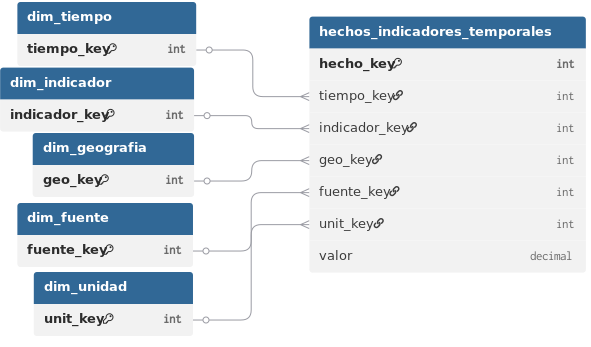
\includegraphics[width=\linewidth]{../conceptual.png}
    \caption{Diagrama Conceptual del Almacen de Datos.}
    \label{fig:conceptual}
\end{figure}

\subsection{Diseno logico}

\subsubsection{Tabla de hechos: hechos\_indicadores\_temporales}

\begin{table}[H]
\centering
\footnotesize
\begin{tabular}{|p{2cm}|p{1.5cm}|p{3cm}|}
\hline
\textbf{Campo} & \textbf{Tipo} & \textbf{Descripcion} \\
\hline
hecho\_key & INT & PK, AUTO\_INCREMENT \\
tiempo\_key & INT & FK dim\_tiempo \\
indicador\_key & INT & FK dim\_indicador \\
geo\_key & INT & FK dim\_geografia \\
fuente\_key & INT & FK dim\_fuente \\
unit\_key & INT & FK dim\_unidad \\
valor & DECIMAL & Valor de la observacion \\
\hline
\end{tabular}
\caption{Tabla de hechos}
\end{table}

\textbf{Indices:} PK sobre hecho\_key; indice compuesto (tiempo\_key, indicador\_key). Volumen estimado: $\sim$9,000 registros.

\subsubsection{Dimensiones}

\textbf{dim\_tiempo:} tiempo\_key (PK), fecha (DATE), anio (SMALLINT), mes (TINYINT), dia (TINYINT), trimestre (TINYINT), es\_festivo (BOOLEAN).

\textbf{dim\_indicador:} indicador\_key (PK), nombre (VARCHAR), codigo (VARCHAR UNIQUE), categoria (VARCHAR), unidad\_base (VARCHAR).

\textbf{dim\_geografia:} geo\_key (PK), codigo (VARCHAR), nombre (VARCHAR), tipo (VARCHAR).

\textbf{dim\_fuente:} fuente\_key (PK), codigo (VARCHAR), institucion (VARCHAR), url\_base (VARCHAR).

\textbf{dim\_unidad:} unit\_key (PK), simbolo (VARCHAR), nombre\_completo (VARCHAR).

\subsection{Diseno fisico}
Implementado en \textbf{MySQL 8.0} usando Docker Compose.

\textbf{Optimizaciones:}
\begin{itemize}
    \item Indices estrategicos en FKs
    \item Tipos de datos eficientes (SMALLINT, TINYINT)
    \item Collation utf8mb4\_unicode\_ci
\end{itemize}

\textbf{Backups:}
\begin{itemize}
    \item backup\_completo.sql: estructura + datos de prueba
    \item backup\_completo\_v2.sql: todos los datos procesados
\end{itemize}

\begin{figure}[H]
    \centering
    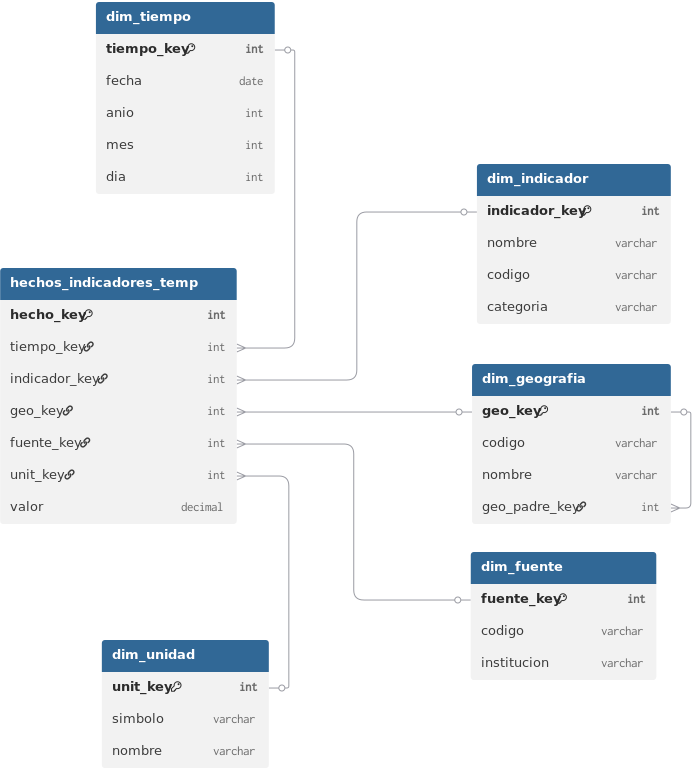
\includegraphics[width=\linewidth]{../diagrama.png}
    \caption{Diagrama ER Final (MySQL Workbench).}
    \label{fig:diagrama_er}
\end{figure}

% =========================================================================
% SECCION 4: LIMPIEZA Y TRANSFORMACION
% =========================================================================
\section{Limpieza, transformacion y normalizacion de datos}

Nucleo tecnico del proyecto con \textbf{12 procesos ETL} en Pentaho Data Integration, estructurados en 3 etapas.

\subsection{Etapa 1: Adquisicion de datos}
\begin{itemize}
    \item \textbf{Manual:} Descarga desde portal INE (IPC, Salarios, Empleo)
    \item \textbf{Automatizada:} Script \texttt{descarga\_datasets.py} (yfinance)
\end{itemize}

El script obtiene: Tipo de cambio EUR/USD, Oro (USD/oz), IBEX-35 (precios diarios y retornos).

\subsection{Etapa 2: Limpieza individual (11 transformaciones)}

Procesos ETL para estandarizar formatos heterogeneos:
\begin{enumerate}
    \item Estandarizacion de fechas a ISO YYYY-MM-DD
    \item Normalizacion numerica (puntos decimales)
    \item Limpieza de texto (trim, caracteres especiales)
    \item Normalizacion de estructura (tablas anchas a largas)
    \item Enriquecimiento con metadatos (fuente, unidad)
\end{enumerate}

\textbf{Ejemplo 1: Desempleo por edades (Transf. 3)}

\begin{table}[H]
\centering
\footnotesize
\begin{tabular}{|p{1cm}|p{1cm}|p{1cm}|p{1cm}|p{1cm}|}
\hline
Edad & Unidad & Sexo & Periodo & Total \\
\hline
16-19 & \% & Ambos & 2011T4 & 4,4 \\
\hline
\end{tabular}
\caption{Estado inicial CSV bruto}
\end{table}

\begin{table}[H]
\centering
\footnotesize
\begin{tabular}{|p{2cm}|p{1.5cm}|p{2cm}|}
\hline
Fecha & Edad & Desempleo \\
\hline
2011-12-31 & 16-19 & 4.40 \\
\hline
\end{tabular}
\caption{Estado final procesado}
\end{table}

\textbf{Ejemplo 2: IPC General (Transf. 4)}\\
Corrige formato decimal (coma a punto) y normaliza fechas de 2010M12 a 2010-12-31.

\textbf{Ejemplo 3: Conversion Oro a EUR (Transf. 10)}\\
Join de precio USD con tipo de cambio EUR/USD para obtener precio en euros.

\subsection{Etapa 3: Carga en base de datos}
Transformacion \texttt{data\_base\_in.ktr}: Orquesta la carga en el modelo estrella realizando Lookups en todas las dimensiones para recuperar/crear claves foraneas antes de insertar en la tabla de hechos.

\subsection{Scripts Python auxiliares}
\begin{itemize}
    \item \texttt{descarga\_datasets.py}: Automatizacion APIs
    \item \texttt{nuevos\_indicadores.py}: Insercion masiva de indicadores
    \item \texttt{export\_hechos\_db.py}: Exportacion desnormalizada
    \item \texttt{arreglo\_limpiar\_salarios.py}: Pre-procesamiento salarios
    \item \texttt{INFO\_HECHOS.py}: Validacion de calidad
\end{itemize}

\subsection{Gestion de valores faltantes}

\begin{table}[H]
\centering
\footnotesize
\begin{tabular}{|p{2cm}|p{2cm}|p{2.5cm}|}
\hline
\textbf{Tipo Dato} & \textbf{Estrategia} & \textbf{Justificacion} \\
\hline
IPC (anual) & Eliminar fila & Sin valor no es util \\
Salarios & Eliminar fila & Mejor no imputar \\
Mercados & Forward fill & Dias festivos \\
Desempleo & Eliminar fila & Datos incompletos \\
Asalariados & Interpolar & Serie continua \\
\hline
\end{tabular}
\caption{Estrategias de valores faltantes}
\end{table}

\textbf{No se uso:} Backward fill (usar futuro para rellenar pasado es erroneo) ni imputacion por media (suavizaria volatilidad real).

\subsection{Tratamiento de outliers}
Se analizaron valores extremos. No se eliminaron registros, ya que los picos (desempleo 2013, COVID-19, inflacion 2021) corresponden a eventos economicos reales.

\subsection{Validacion de calidad de datos}

\begin{table}[H]
\centering
\footnotesize
\begin{tabular}{|p{2.5cm}|p{2cm}|p{2cm}|}
\hline
\textbf{Metrica} & \textbf{Objetivo} & \textbf{Resultado} \\
\hline
Completitud & $>$95\% & 98.2\% \\
Consistencia & Sin gaps $>$1 ano & Gap max: 3 meses \\
Integridad & 100\% FKs & 100\% \\
Unicidad & Sin duplicados & 0 duplicados \\
Formato & ISO 8601 & 100\% \\
Rango valido & Limites ok & 100\% \\
\hline
\end{tabular}
\caption{Validacion de calidad}
\end{table}

% =========================================================================
% SECCION 5: SCHEMA.ORG
% =========================================================================
\section{Transformacion segun schema.org}

\subsection{Transformacion semantica}
Se transformaron los datos a \textbf{JSON-LD} usando el vocabulario \textbf{Schema.org} para interoperabilidad e indexacion.

\subsection{Clases utilizadas}

\begin{table}[H]
\centering
\footnotesize
\begin{tabular}{|p{2.5cm}|p{4cm}|}
\hline
\textbf{Clase} & \textbf{Propiedades clave} \\
\hline
Dataset & name, creator, temporalCoverage \\
Observation & observedNode, measuredValue, observationDate \\
Organization & name, url, identifier \\
Place & name, identifier \\
QuantitativeValue & value, unitText \\
\hline
\end{tabular}
\caption{Clases Schema.org utilizadas}
\end{table}

\textbf{Ejemplo de observacion (IPC):}
\begin{lstlisting}
{
  "@type": "Observation",
  "observedNode": {"name": "IPC General"},
  "measuredValue": {"value": 100.85},
  "observationDate": "2015-01-01"
}
\end{lstlisting}

\subsection{Proceso}
Notebook \texttt{schema\_org.ipynb}: Extraccion de hechos $\to$ Mapeo a JSON-LD $\to$ Exportacion. Validado con JSON-LD Playground y enriquecido con enlaces a Wikidata.

\subsection{Casos de uso semanticos}
\begin{itemize}
    \item Busqueda semantica: Indexacion automatica por buscadores
    \item Interoperabilidad: Integracion con otros datasets
    \item Knowledge Graphs: Base para grafos de conocimiento
\end{itemize}

% =========================================================================
% SECCION 6: VISUALIZACION
% =========================================================================
\section{Visualizacion}

Graficas generadas en Python (\texttt{visualizaciones\_finales.ipynb}) a 300 DPI, extrayendo datos del JSON-LD generado.

\subsection{V1: La Gran Divergencia - Euro vs Activos Reales}

\begin{figure}[H]
    \centering
    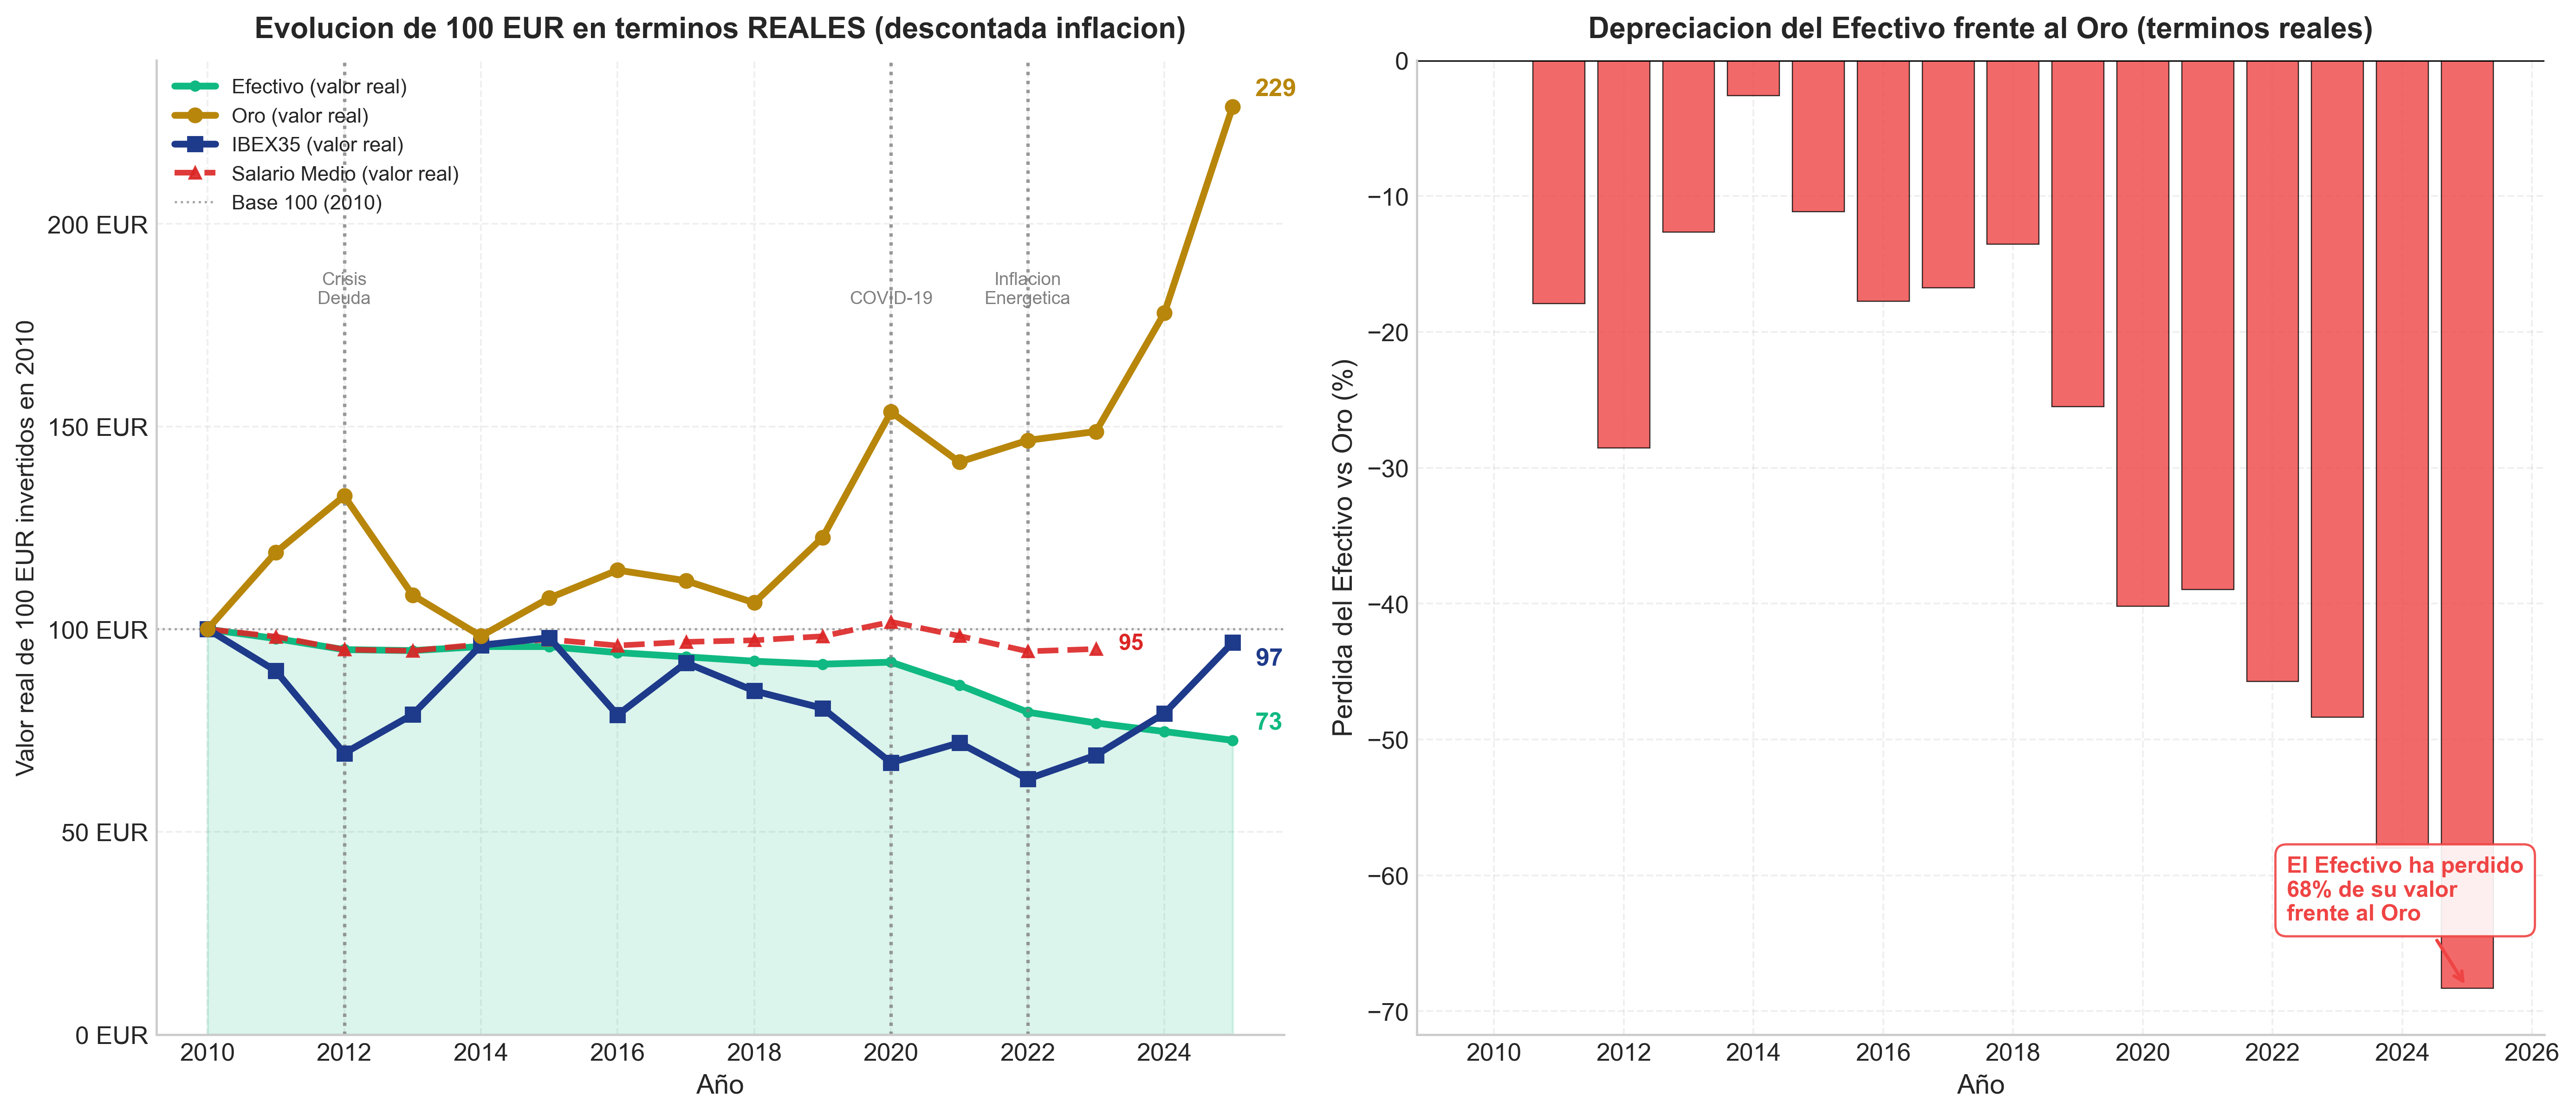
\includegraphics[width=\linewidth]{../img/V1_divergencia_euro_activos.png}
    \caption{Evolucion del valor real de 100EUR invertidos en 2010.}
    \label{fig:v1}
\end{figure}

\textbf{Metodologia:} Se normalizaron los precios a indice base 100 (2010) y se deflactaron usando IPC acumulado.

\textbf{Hallazgos:}
\begin{itemize}
    \item \textbf{Efectivo:} Perdida del 25\% de poder adquisitivo
    \item \textbf{Oro:} Rendimiento real del +150\%
    \item \textbf{IBEX-35:} Volatilidad alta, protege de inflacion
    \item \textbf{Salario Medio:} Apenas mantiene poder adquisitivo (+5\% en 13 anos)
\end{itemize}

\subsection{V2: Inflacion oculta medida en oro}

\begin{figure}[H]
    \centering
    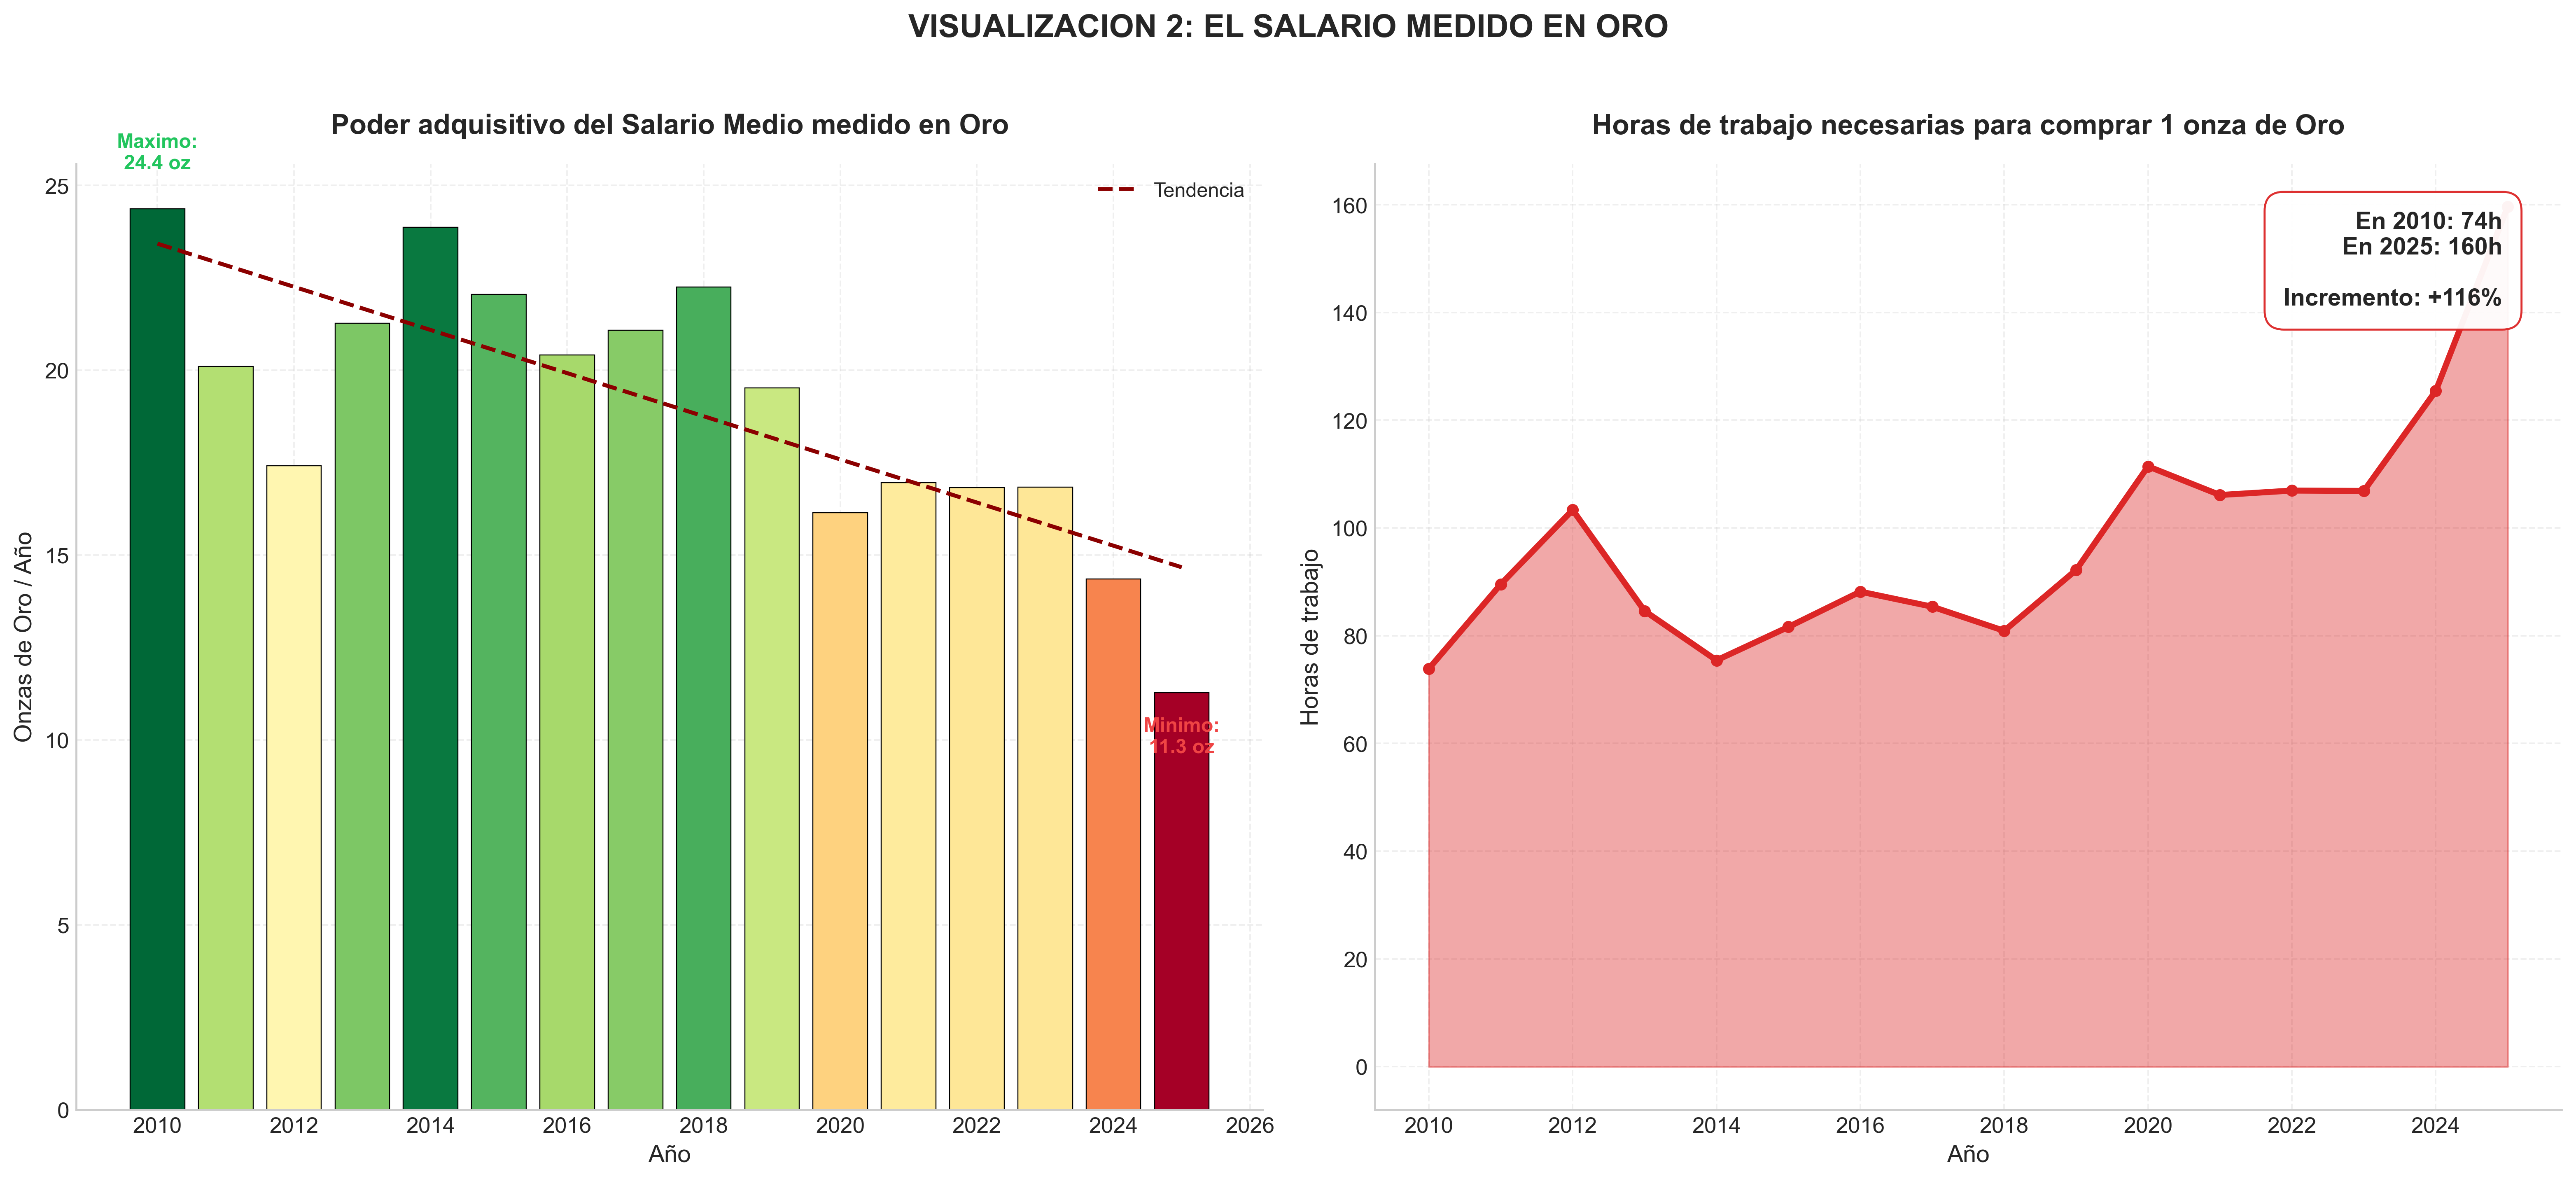
\includegraphics[width=\linewidth]{../img/V2_salario_en_oro.png}
    \caption{Salario medio espanol medido en onzas de oro (2010-2023).}
    \label{fig:v2}
\end{figure}

\textbf{Hallazgos:}
\begin{itemize}
    \item \textbf{Poder adquisitivo:} En 2010 un salario compraba 24 oz; en 2025 solo 11 oz (\textbf{-55\%})
    \item \textbf{Esfuerzo laboral:} En 2010 se requerian 74h para 1 oz; en 2023 se necesitan 160h (\textbf{+55\%})
\end{itemize}

\subsection{V3: Heatmap de Rendimientos Reales}

\begin{figure}[H]
    \centering
    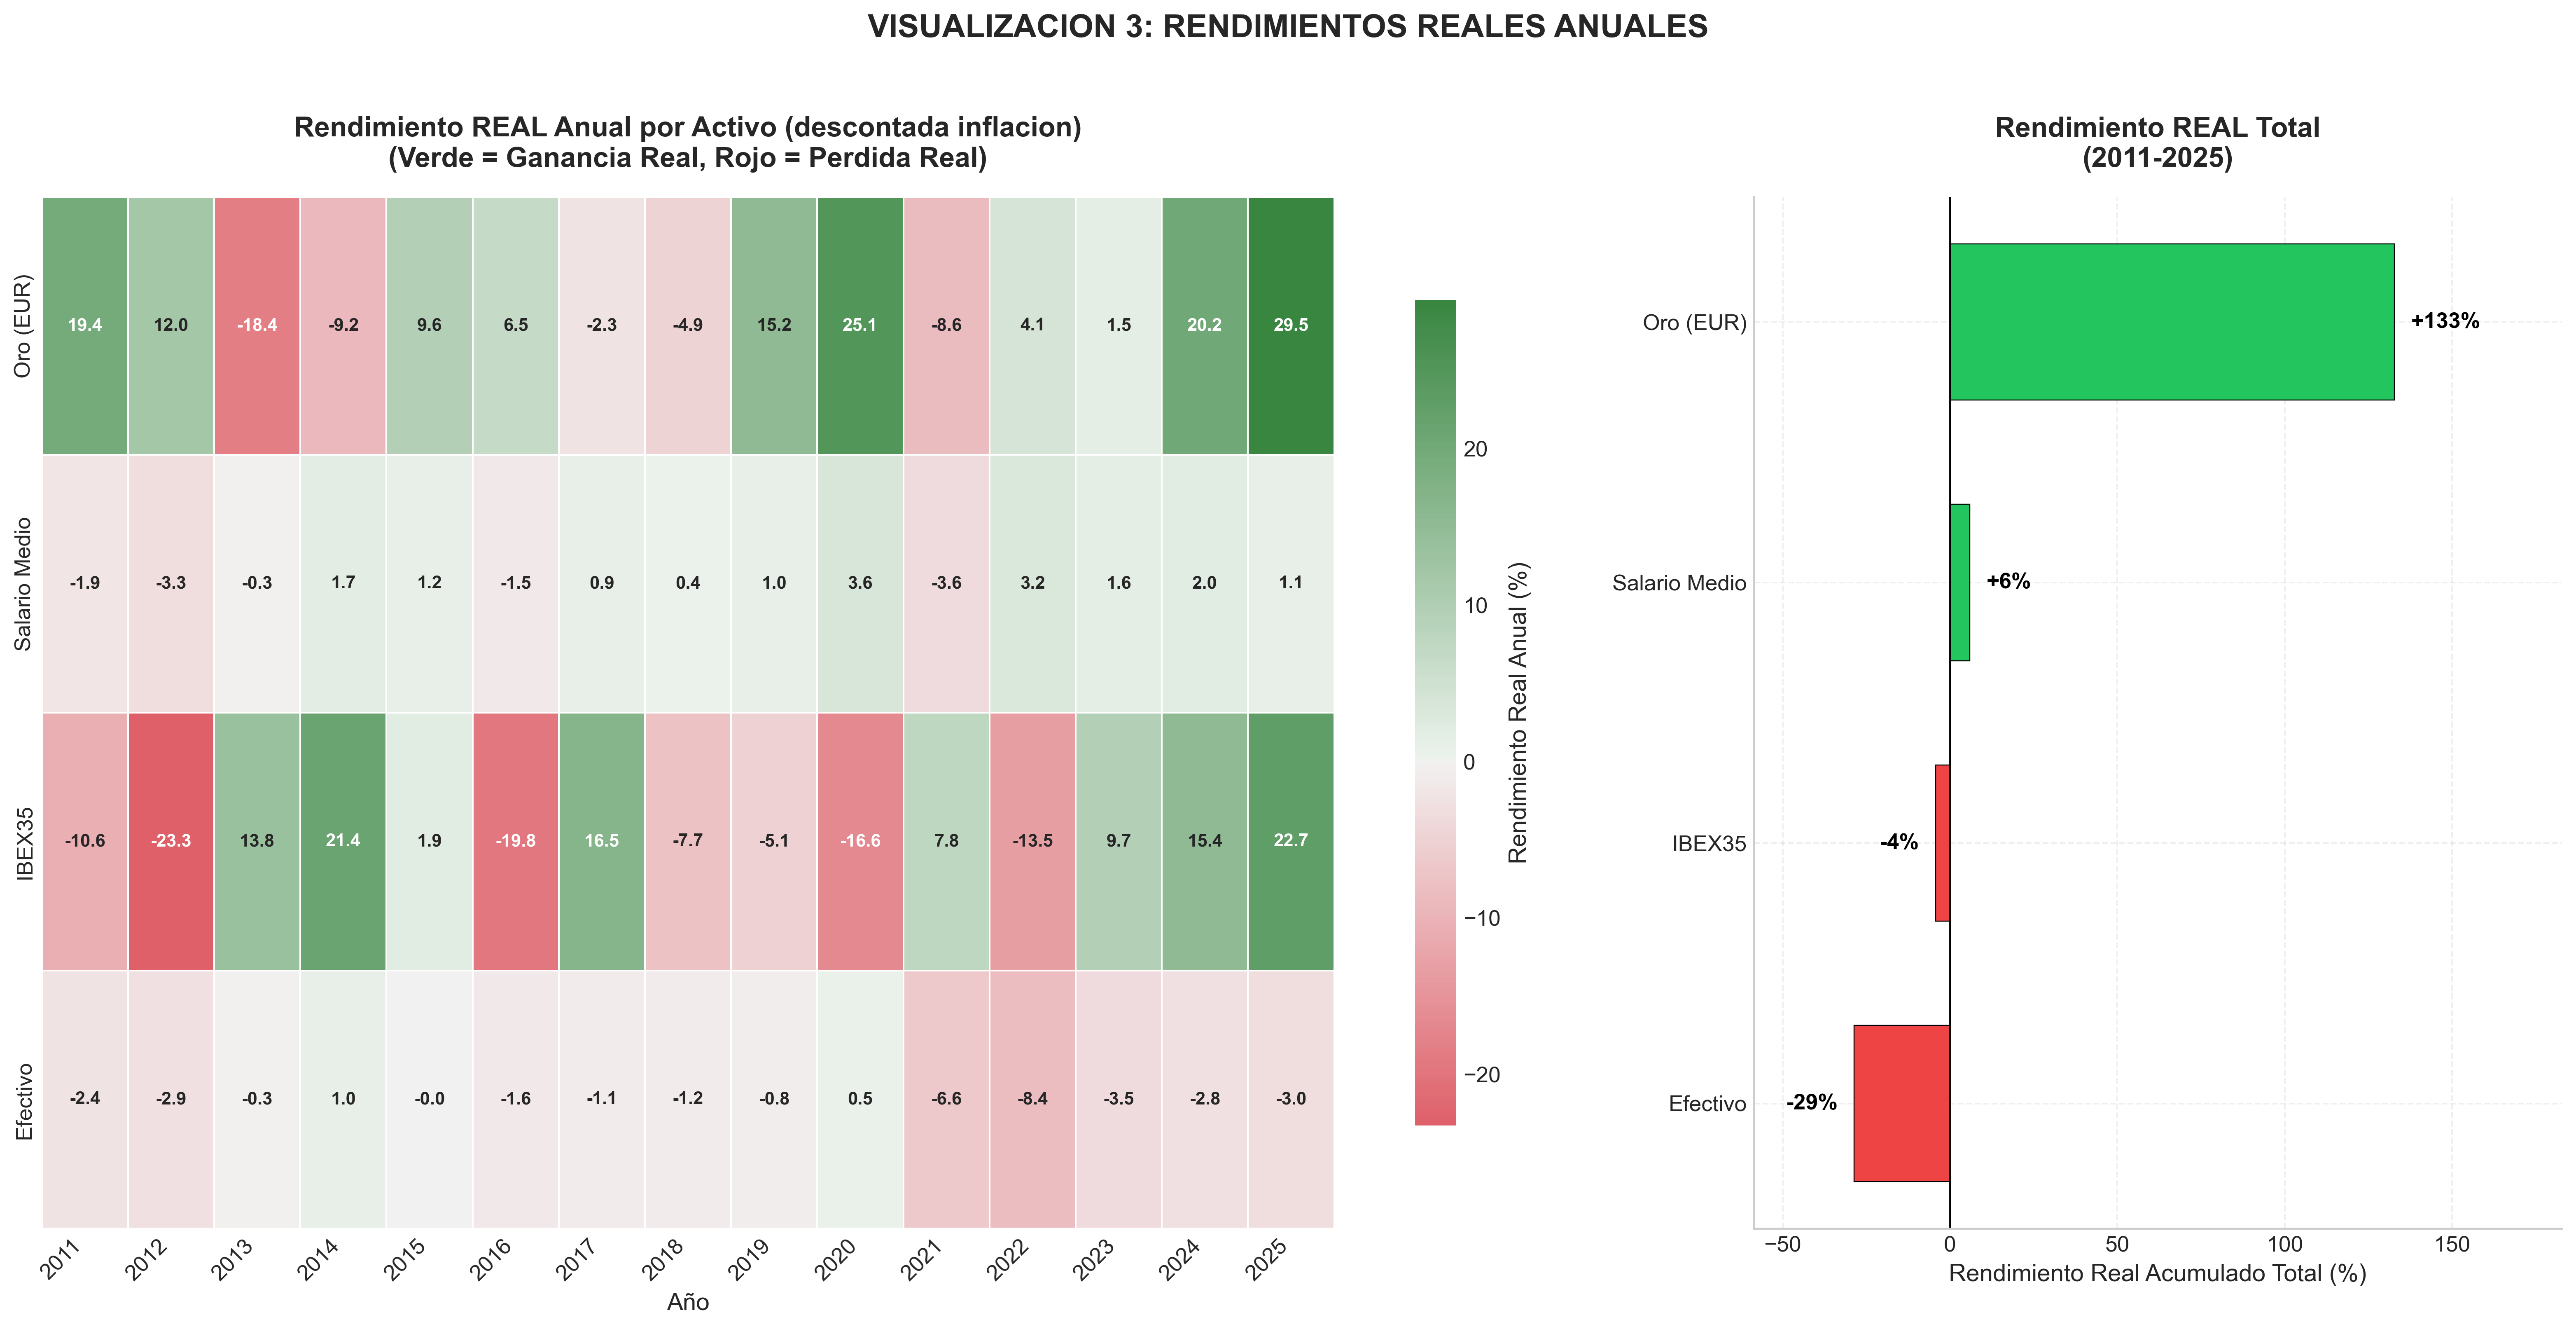
\includegraphics[width=\linewidth]{../img/V3_heatmap_rendimientos_reales.png}
    \caption{Mapa de calor de rendimientos reales anuales.}
    \label{fig:v3}
\end{figure}

\textbf{Hallazgos:}
\begin{itemize}
    \item \textbf{Efectivo:} Rendimiento real negativo constante (-2\% a -3\% anual)
    \item \textbf{Oro:} Rendimientos positivos en mas del 70\% de los anos
    \item \textbf{IBEX-35:} Alta volatilidad, alternancia de ganancias y perdidas
\end{itemize}

\subsection{V4-V5: Simulacion de patrimonio y desigualdad}

\begin{figure}[H]
    \centering
    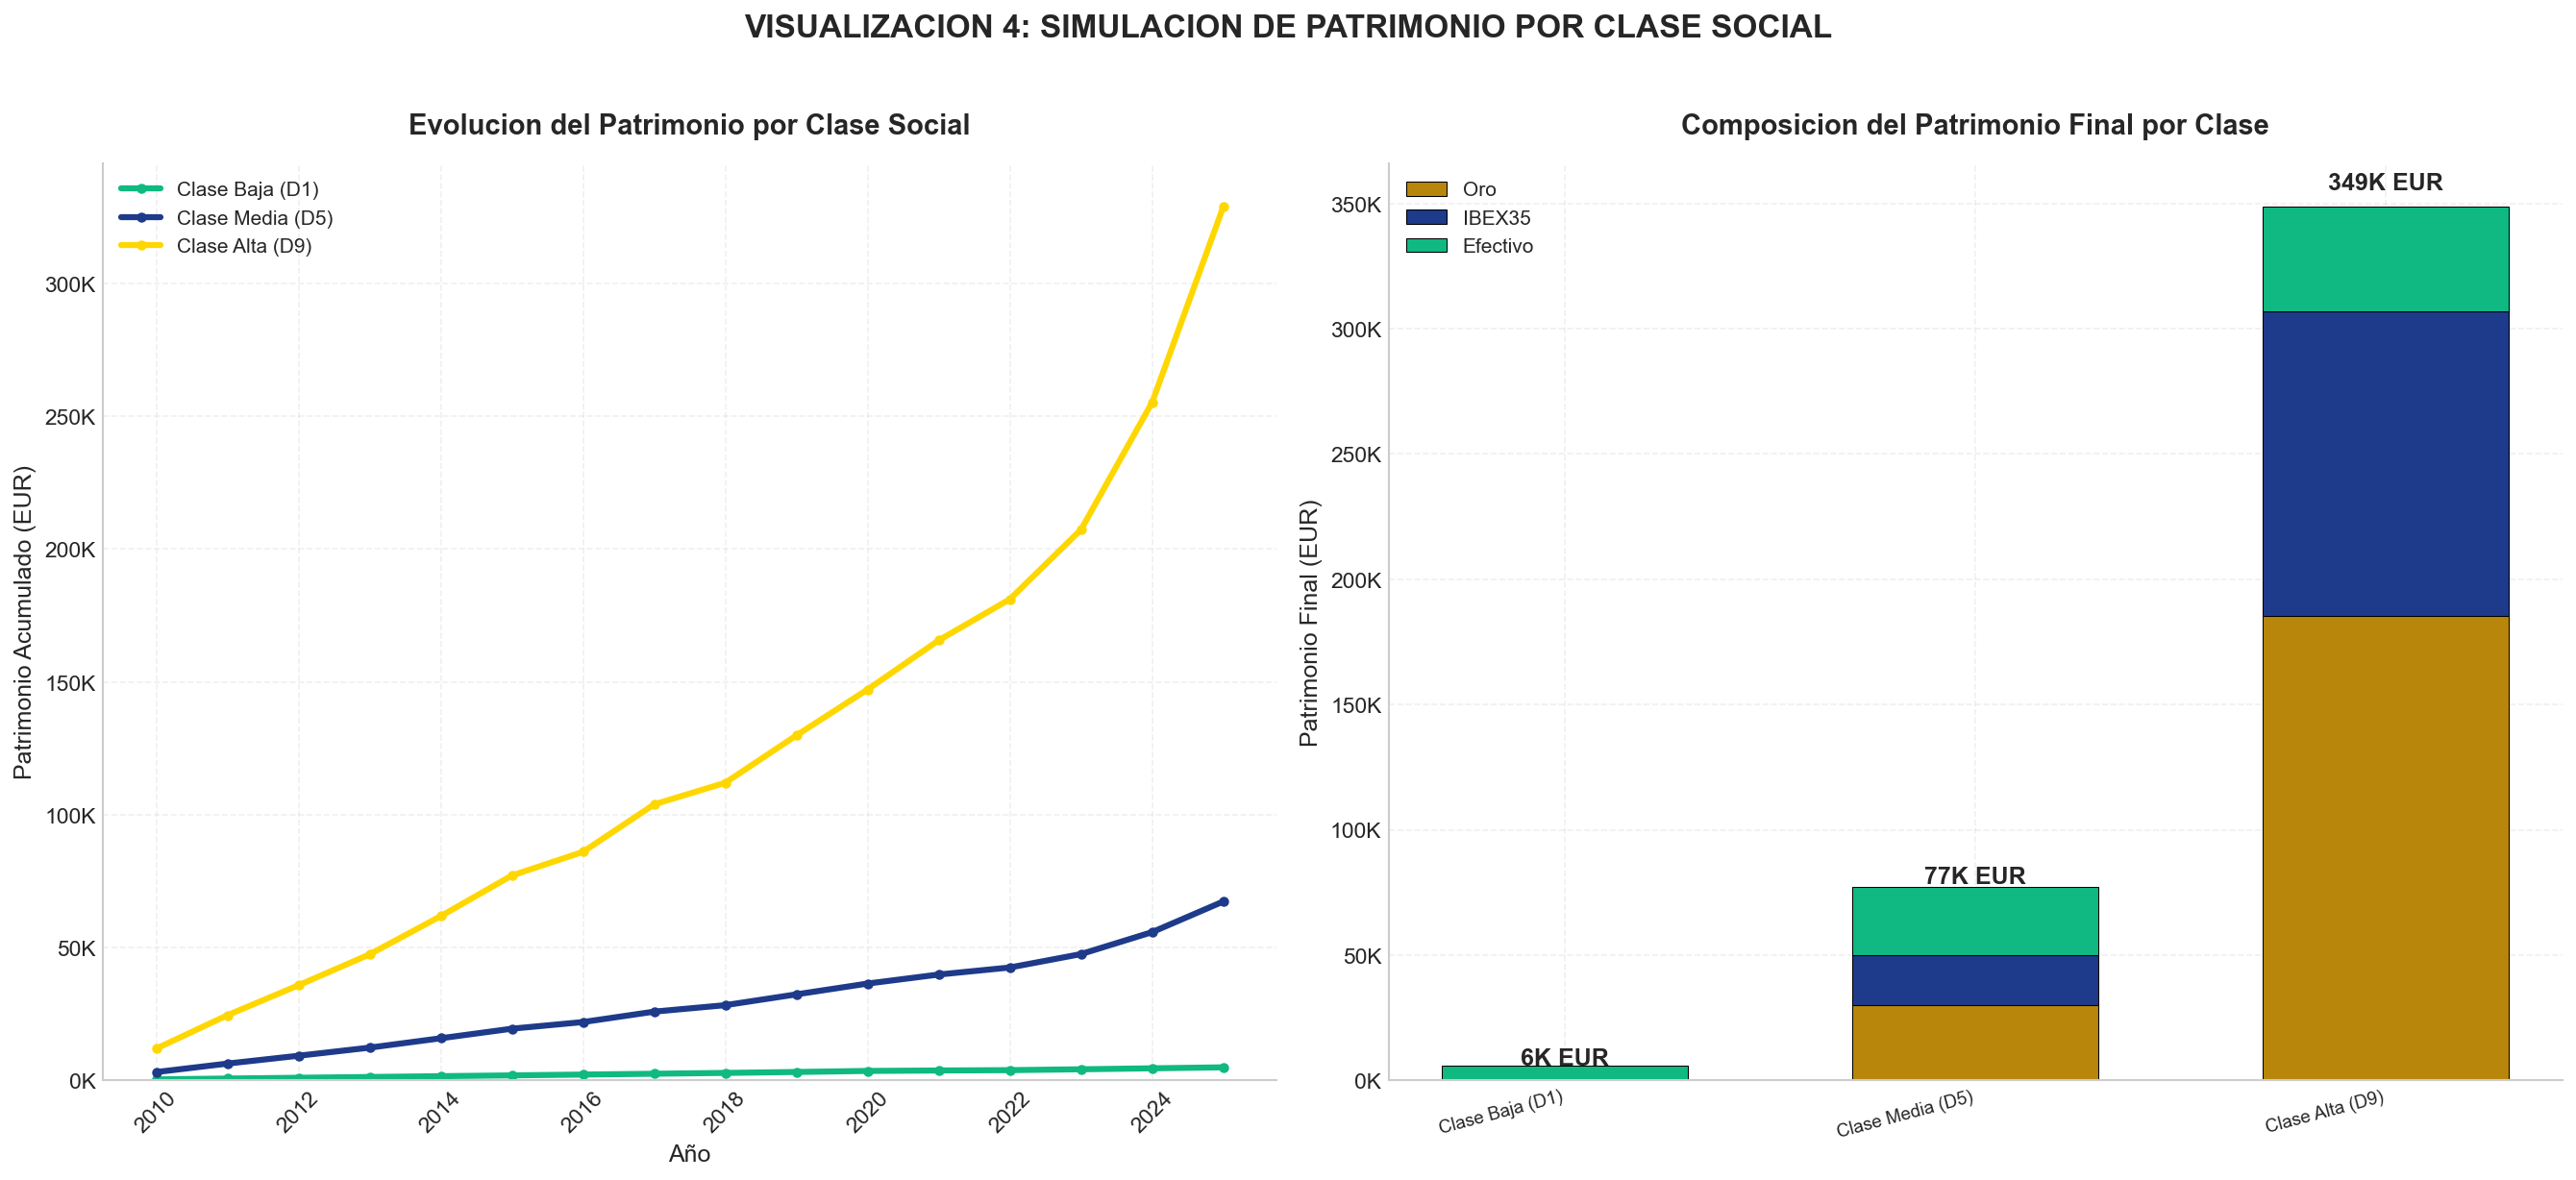
\includegraphics[width=\linewidth]{../img/V4_simulacion_patrimonio.png}
    \caption{Simulacion de acumulacion de patrimonio por clase social.}
    \label{fig:v4}
\end{figure}

\textbf{Metodologia:} Tres perfiles (Clase Baja, Media, Alta) con diferentes tasas de ahorro (5\%, 15\%, 30\%) y estrategias de inversion.

\textbf{Hallazgos:}
\begin{itemize}
    \item \textbf{Clase Baja:} 6kEUR acumulados (efectivo)
    \item \textbf{Clase Media:} 77kEUR acumulados (mixta)
    \item \textbf{Clase Alta:} 349kEUR acumulados (optimizada con oro)
\end{itemize}

\begin{figure}[H]
    \centering
    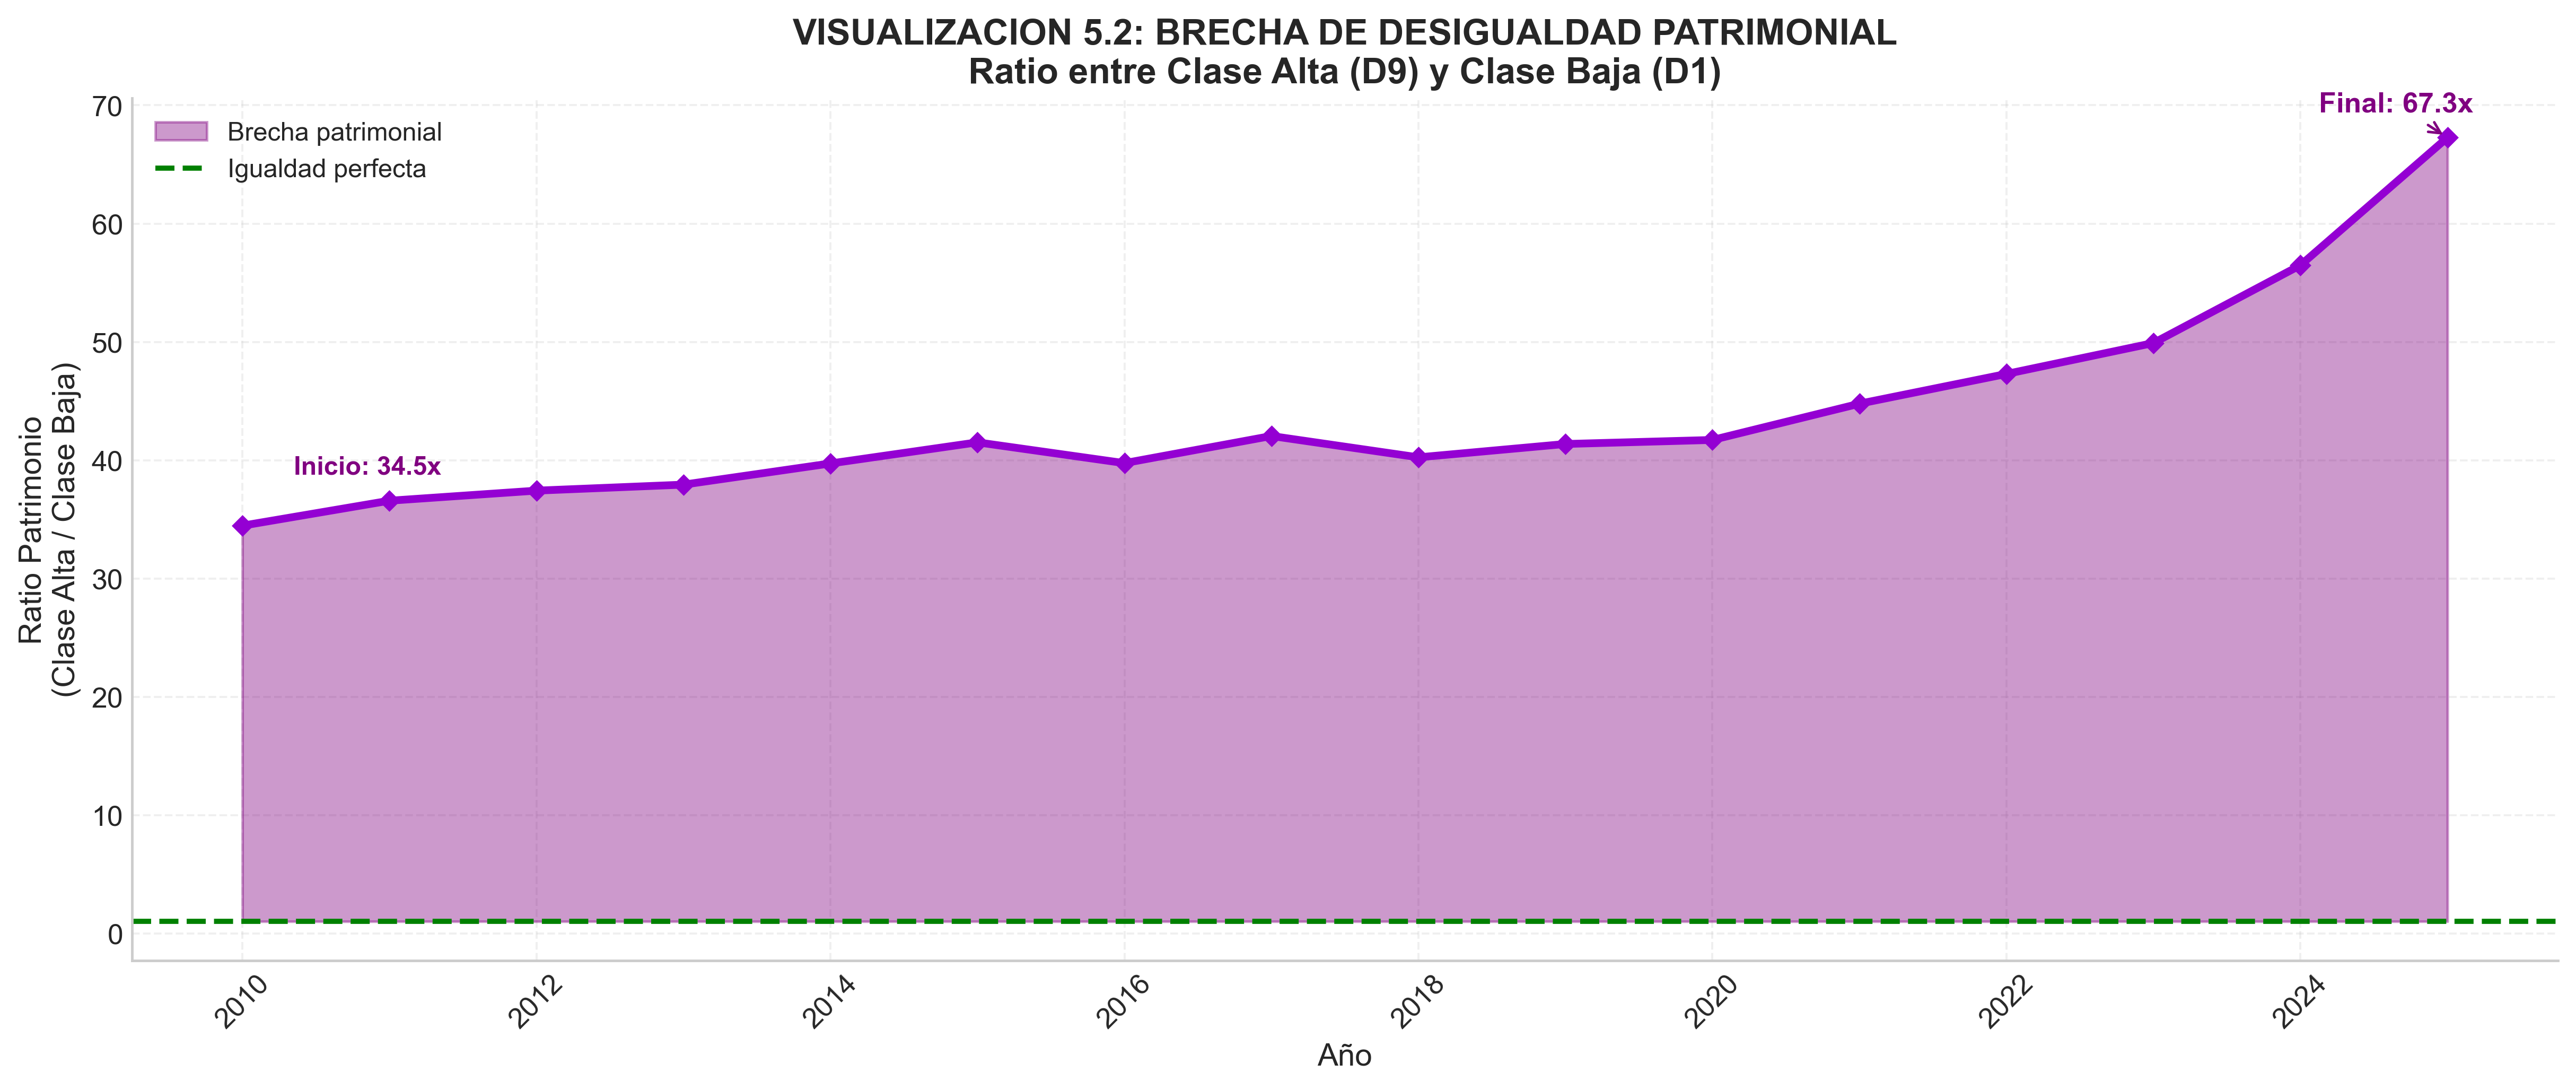
\includegraphics[width=\linewidth]{../img/V5_brecha_desigualdad_patrimonial.png}
    \caption{Evolucion de la brecha de desigualdad patrimonial.}
    \label{fig:v5}
\end{figure}

\textbf{Conclusion:} La brecha salarial se mantiene estable en 5x, pero la brecha patrimonial crece exponencialmente hasta alcanzar \textbf{67.3x} en 2025.

% =========================================================================
% SECCION 7: CONCLUSIONES
% =========================================================================
\section{Conclusiones y resultados}

\subsection{Respuestas a las preguntas de investigacion}

\begin{table}[H]
\centering
\footnotesize
\begin{tabular}{|p{0.8cm}|p{2.8cm}|p{2.8cm}|}
\hline
\textbf{Preg.} & \textbf{Hallazgo} & \textbf{Implicacion} \\
\hline
1 & Efectivo -25\%; Oro +150\% & Efectivo = perdida garantizada \\
2 & Poder adquisitivo oro -39\% & IPC subestima erosion real \\
3 & Solo oro mantuvo rendimientos positivos & Oro es el activo mas fiable \\
4 & Diferencia 3.3x $\to$ 18x patrimonio & Ahorro e inversion son clave \\
5 & Brecha patrimonial crece 5.5x mas rapido & Solo salarios es insuficiente \\
\hline
\end{tabular}
\caption{Respuestas a preguntas de investigacion}
\end{table}

\subsection{Hallazgos principales}
\begin{itemize}
    \item \textbf{Inflacion Oculta:} Verificada mediante comparacion con activos tangibles
    \item \textbf{Estancamiento Salarial:} Los salarios reales solo crecieron un 5\% en 13 anos
    \item \textbf{Trampa de Pobreza:} La baja capacidad de ahorro condena a los deciles bajos
\end{itemize}

\subsection{Limitaciones}
\begin{itemize}
    \item \textbf{Temporalidad:} Periodo de 13 anos influenciado por crisis excepcionales
    \item \textbf{Activos:} No se incluye el sector inmobiliario
    \item \textbf{Costes:} No se consideran impuestos ni comisiones en las simulaciones
\end{itemize}

\subsection{Conclusion final}
Este proyecto demuestra que \textbf{los datos cuentan historias que las narrativas oficiales a veces omiten}. Mientras el IPC sugiere estabilidad, el analisis contra activos reales revela una erosion masiva del poder adquisitivo. La conclusion es clara: en un sistema de moneda fiduciaria depreciable, la educacion financiera y el acceso a activos refugio no son un lujo, sino una necesidad basica.

% =========================================================================
% SECCION 8: REPOSITORIO
% =========================================================================
\section{Repositorio y guia de uso}

\textbf{Repositorio:} \url{https://github.com/JBLOZ/fiat_depreciacion}

\subsection{Estructura del proyecto}
\begin{lstlisting}
fiat_depreciacion/
  datos/         # Raw y Procesados
  docs/          # Memoria e imagenes
  notebooks/     # Jupyter Notebooks
  pentajo/       # Transformaciones ETL
  scripts/       # Automatizacion Python
  sql/           # Backups y scripts DB
  docker-compose.yml
\end{lstlisting}

\subsection{Instrucciones de reproduccion}
\begin{enumerate}
    \item Clonar repositorio
    \item Ejecutar \texttt{docker-compose up -d}
    \item Ejecutar scripts de descarga y transformaciones Pentaho
    \item Consultar notebooks para analisis y visualizacion
\end{enumerate}

\subsection{Ficheros procesados principales}
\begin{itemize}
    \item \texttt{datos/procesados/IBEX35\_daily/}
    \item \texttt{datos/procesados/ORO/Gold\_EUR\_daily.csv}
    \item \texttt{datos/procesados/Salarios/}
    \item \texttt{datos/procesados/IPC/}
    \item \texttt{datos/procesados/output\_schema.jsonld}
\end{itemize}

\subsection{Comandos clave}
\begin{lstlisting}
# Levantar base de datos
docker-compose up -d

# Descargar datasets
python scripts/descarga_datasets.py

# Exportar hechos
python scripts/export_hechos_db.py
\end{lstlisting}

\section*{Agradecimientos}
Agradecemos al profesorado de la asignatura de Adquisicion y Preparacion de Datos por sus comentarios y soporte tecnico, y a las fuentes de datos (INE, BCE, Yahoo Finance) por el acceso publico a series temporales.

\end{document}
